\section{Laser Sensor}
The laser sensor can be modelled as a first-order system with a transfer function of the form $F(S)=\frac{K}{{\tau}s+1}$, and K is the static gain of the system and $\tau$ is the time constant of the system. First-order systems are very common in engineering applications, in practical applications, control systems can be designed based on the transfer function of the laser sensor to achieve the desired control objectives. In this case, the laser sensor is used to regulate the negative feedback in order to improve the performance and stability of the system.
\subsection*{Derivation} \hfill \\
\noindent The sensor can be described by the first-order differential equation 
\begin{equation}
a_{\text{0}}x+a_{\text{1}}\dot{x}=bu
\end{equation}
\noindent From the questions $a_{\text{0}}\neq0$
\begin{equation}
x+\frac{a_{\text{1}}}{a_{\text{0}}}\dot{x}=\frac{b}{a_{\text{0}}}u
\end{equation}
\noindent Substitute time constant $\tau=\frac{a_{\text{1}}}{a_{\text{0}}}$ and static gain $K=\frac{b}{a_{\text{0}}}$ into the equation.
\begin{equation}
x+\tau\dot{x}=Ku
\end{equation}
\noindent Apply the Laplace transform on the both sides of the equation assuming zero initial conditions
\begin{equation}
(1+{\tau}s)X(s)=KU(s)
\end{equation}
\noindent Therefore, the transfer function of the sensor is
\begin{equation}
G(s)=\frac{X(s)}{U(s)}=\frac{K}{{\tau}s+1}
\end{equation}
\subsection*{Block Diagram} \hfill \\
where $\tau$ is 30 ms, K is 1
\begin{figure}[ht]
    \centering
    \begin{minipage}{0.49\textwidth}
        \centering
        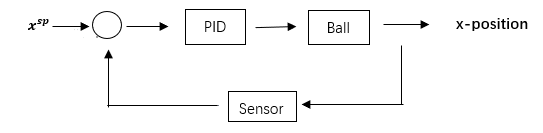
\includegraphics[width=1.0\linewidth]{Laser Sensor/All Control System.png}
        \caption{The complete control system }
    \end{minipage}
\end{figure}